\chapter{进程管理}

\section{进程}

\subsection{进程(Process)}

Windows任务管理器提供了有关计算机性能的信息,并显示了计算机上所运行的程序和进程的详细信息。

\begin{figure}[H]
	\centering
	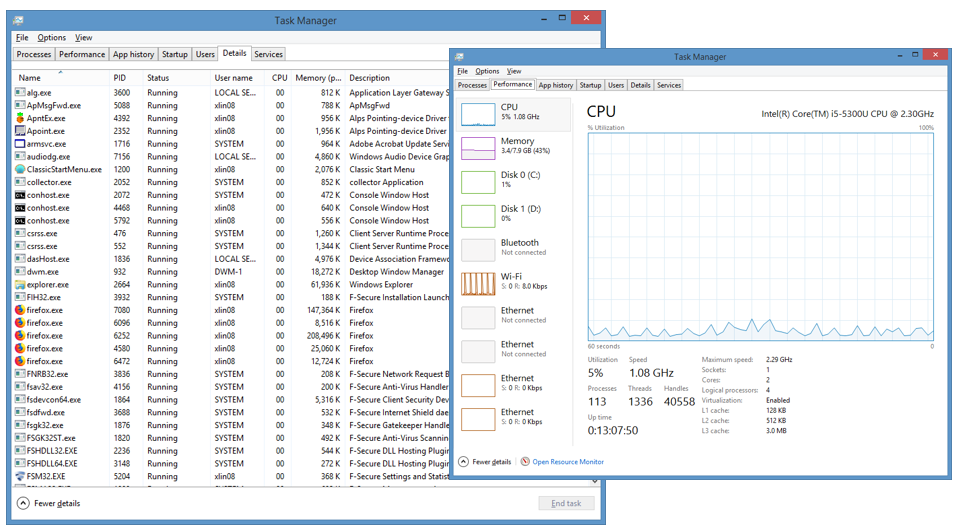
\includegraphics[scale=0.6]{img/C2/2-1/1.png}
	\caption{Windows进程}
\end{figure}

进程指的是一个具有一定独立功能的程序关于某个数据集合的一次运行活动。进程是系统进行资源分配和调度运行的基本单位。进程实体中包含三个组成部分:

\begin{enumerate}
	\item 程序
	\item 数据
	\item 进程控制块(PCB, Process Control Block)
\end{enumerate}

程序(program)与进程是有区别的,程序是静态的,进程是动态的。当程序的可执行文件被装入内存后就会变成进程。进程可以认为是执行中的程序,进程需要一定资源(如CPU时间、内存、文件、I/O设备)完成任务。这些资源可以在创建的时候或者运行中分配。一个程序可以通过GUI(Graphic User Interface)图形用户界面的鼠标点击、CLI(Command-line Interface)命令行界面输入程序名等方式运行。

\begin{figure}[H]
	\centering
	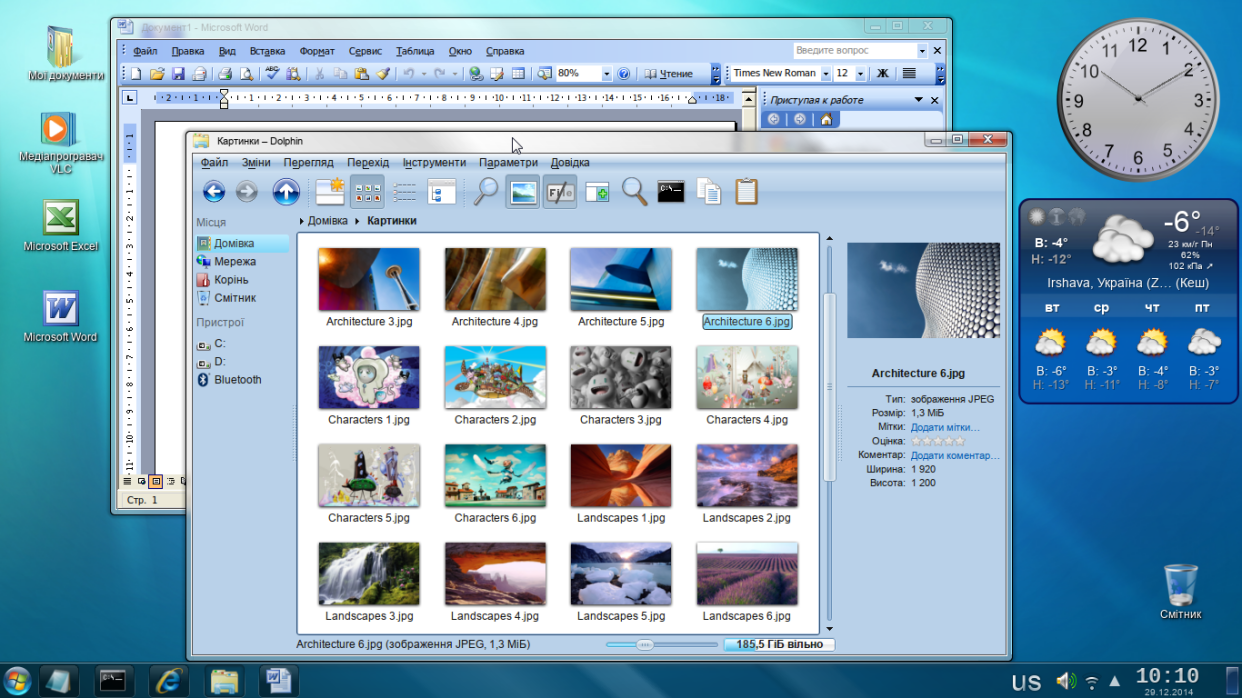
\includegraphics[]{img/C2/2-1/2.png}
	\caption{GUI图形用户界面}
\end{figure}

\begin{figure}[H]
	\centering
	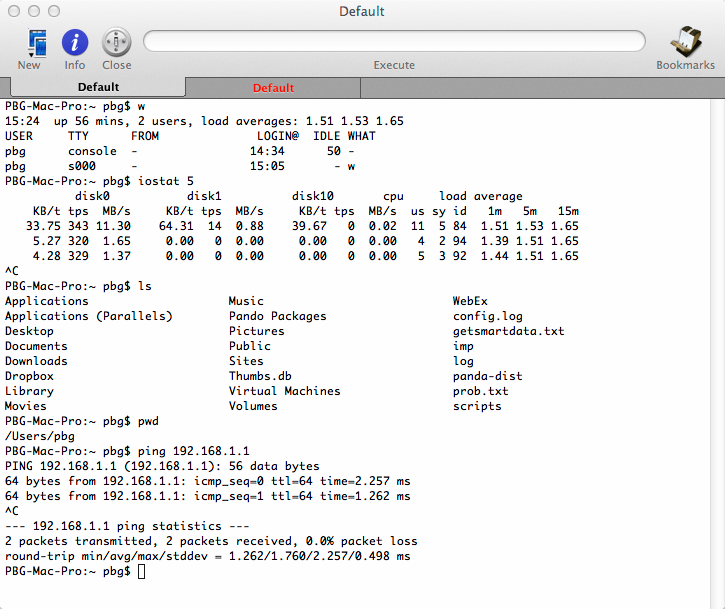
\includegraphics[scale=0.5]{img/C2/2-1/3.png}
	\caption{CLI命令行界面}
\end{figure}

\subsection{内存管理}

内存通常包括了栈区(stack)、堆区(heap)、数据区、程序代码区:

\begin{itemize}
	\item 栈区:由编译器自动分配和释放,存放函数的参数值、局部变量的值等。

	\item 堆区:一般由程序员分配和释放,若程序员不释放,程序结束后被OS回收。

	\item 数据区:存放全局变量和静态变量,程序结束后由系统释放。

	\item 程序代码区:存放函数体的二进制代码。
\end{itemize}

\begin{figure}[H]
	\centering
	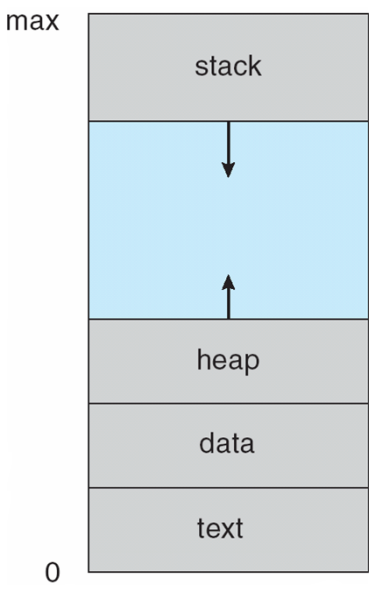
\includegraphics[]{img/C2/2-1/4.png}
	\caption{内存管理}
\end{figure}

\subsection{进程状态模型}

在两状态进程模型中,进程被分为运行态(running)和非运行态(not-running)。

\begin{figure}[H]
	\centering
	\begin{tikzpicture}[node distance=3cm,thick,auto]
		\node[state,initial] (s1) {非运行态};
		\node[state,accepting right,accepting text = {end}] (s2) [right of=s1] {运行态};

		\path[->] (s1) edge[bend left] node[above] {分配} (s2);
		\path[->] (s2) edge[bend left] node[below] {暂停} (s1);
	\end{tikzpicture}
	\caption{两态模型}
\end{figure}

并非所有进程只要是非运行态就一定处于就绪状态,有的需要阻塞等待I/O完成。因此非运行态又可分为就绪态(ready)和阻塞态(block)。 \\

所有的进程从其创建到销毁都有各自的生命周期,进程要经过如下几个阶段:

\begin{figure}[H]
	\centering
	\begin{tikzpicture}[node distance=4.5cm,thick,auto]
		\node[state,initial] (s1) {创建};
		\node[state] (s2)[below of=s1] {就绪};
		\node[state] (s3)[right of=s2] {执行};
		\node[state] (s4)[above of=s3] {阻塞};
		\node[state,accepting below,accepting text = {end}] (s5)[right of=s3] {释放};

		\path[->] (s1) edge node[left] {许可} (s2);
		\path[->] (s2) edge[bend left] node[above] {CPU调度} (s3);
		\path[->] (s3) edge[bend left] node[below] {时间片执行完} (s2);
		\path[->] (s3) edge node[right] {产生阻塞事件} (s4);
		\path[->] (s4) edge node[left] {解除阻塞} (s2);
		\path[->] (s3) edge node {终止} (s5);
	\end{tikzpicture}
	\caption{五态模型}
\end{figure}

\begin{enumerate}
	\item 创建状态:系统已经为其分配了PCB(可以获取进程的而信息),但是所需要执行的进程的上下文环境(context)还未分配,所以这个时候的进程还无法被调度。
	
	\item 就绪状态:该进程已经分配到除CPU之外的全部资源,并等待CPU调度。
	
	\item 执行状态:进程已获得CPU资源,开始正常提供服务。
	
	\item 阻塞状态:所有的进程不可能一直抢占CPU,依据资源调度的算法,每一个进程运行一段时间之后,都需要交出当前的CPU资源,给其它进程执行。
	
	\item 终止状态:某一个进程达到了自然终止的状态,或者进行了强制性的停止,那么进程将进入到终止状态,进程将不再被执行。
\end{enumerate}

\subsection{多进程}

Python中在进行多进程开发的时候可以使用\lstinline|multiprocessing|模块进行多进程的编写,这个模块内容提供有一个\lstinline|Process|类,利用这个类可以进行多进程的定义。所有的Python程序执行都是通过主进程开始的,所有通过\lstinline|Process|定义的进程都属于子进程。

\begin{lstlisting}[language=Python, title=创建多进程]
import multiprocessing

def worker():
	"""
		进程处理函数
	"""
	print("【进程】id:%d,名称:%s" % (
		multiprocessing.current_process().pid,
		multiprocessing.current_process().name)
	)

def main():
	print("【主进程】id:%d,名称:%s" % (
		multiprocessing.current_process().pid,
		multiprocessing.current_process().name)
	)

	# 创建3个进程
	for i in range(3):
		process = multiprocessing.Process(
			target=worker, name="进程%d" % i
		)
		process.start()

if __name__ == "__main__":
	main()
\end{lstlisting}

\begin{tcolorbox}
	\mybox{运行结果} \\
	【主进程】id:4476,名称:MainProcess \\
	【进程】id:14216,名称:进程0 \\
	【进程】id:1424,名称:进程1 \\
	【进程】id:16636,名称:进程2
\end{tcolorbox}

\lstinline|psutil|是一个进程管理的第三方模块,该模块可以跨平台(Linux、UNIX、MaxOS、Windows都支持)地进行进程管理,可以极大地简化不同系统中的进程处理操作。

\begin{lstlisting}[language=Python, title=获取全部进程信息]
import psutil

def main():
	# 获取全部进程
	for process in psutil.process_iter():
		print("【进程】id:%d,名称:%s,创建时间:%s" % (
			process.pid, process.name,
			process.create_time())
		)

if __name__ == "__main__":
	main()
\end{lstlisting}

\newpage

\section{进程控制块PCB}

\subsection{PCB(Process Control Block)}

进程控制块PCB是OS控制和管理进程时所用的基本数据结构,PCB是相关进程存在于系统中的唯一标志,系统根据PCB而感知相关进程的存在。 \\

PCB中包含了关于进程的一些信息,如进程标识(pid)、程序计数器、状态信息、CPU调度信息、内存管理信息、I/O状态信息等。 \\

Linux中C语言\lstinline|<linux/sched.h>|头文件中定义的进程结构如下:

\begin{lstlisting}[language=C, title=进程结构]
pid t_pid;					/* process identifier */
long state;					/* state of the process */
unsigned int time_slice;	/* scheduling information */
struct task_struct *parent;	/* this process's parent */
struct list_head children;	/* this process's children */
struct files_struct *files;	/* list of open files */
struct mm_struct *mm;		/* address space */
\end{lstlisting}

\subsection{进程切换}

当CPU切换到另一个进程时,系统必须保存当前执行进程的上下文(context),并且加载需要被执行进程的上下文。进程的上下文都被保存在PCB中。

\begin{figure}[H]
	\centering
	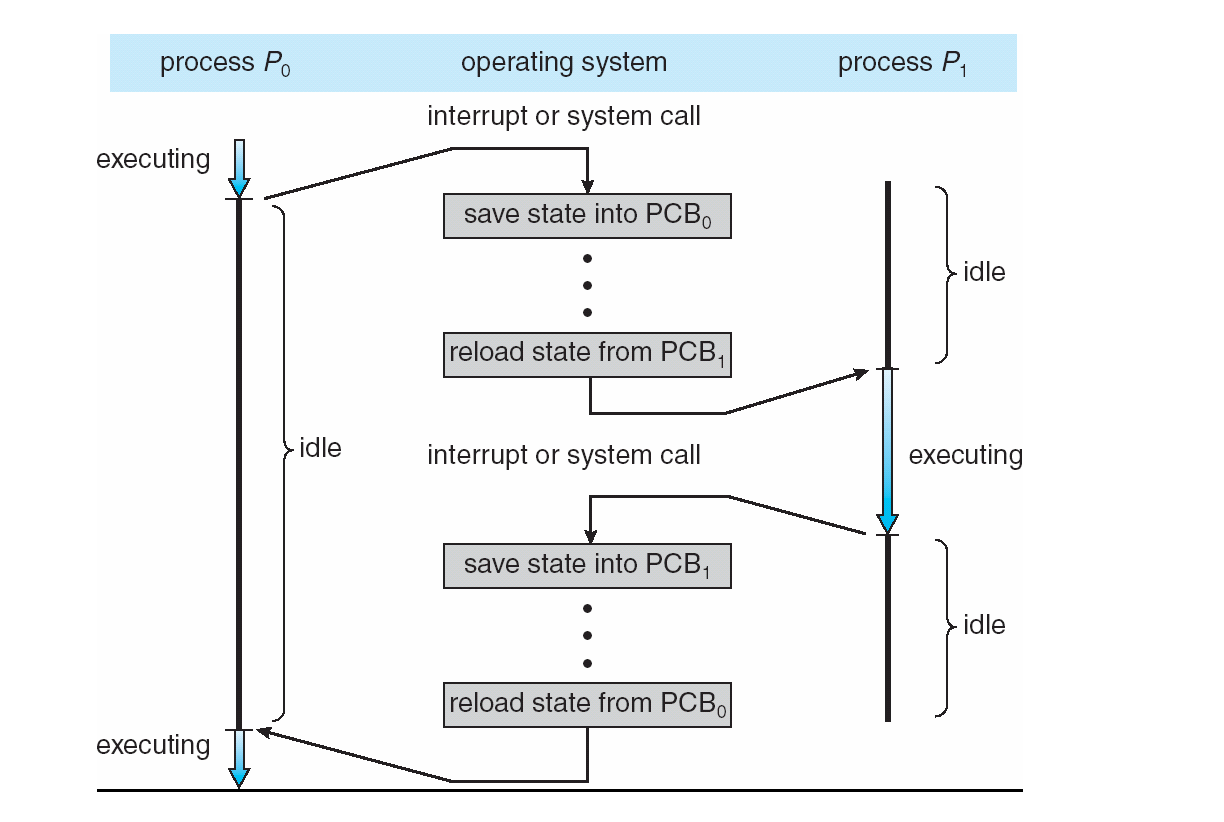
\includegraphics[scale=0.5]{img/C2/2-2/1.png}
	\caption{进程切换}
\end{figure}

\newpage

\section{线程}

\subsection{线程(Thread)}

60年代,在OS中能拥有资源和独立运行的基本单位是进程,然而随着计算机技术的发展,进程出现了很多弊端。由于进程是资源拥有者,创建、撤消与切换存在较大的时空开销。因此在80年代,出现了能独立运行的基本单位线程。 \\

线程是操作系统进行运算调度的最小单位,它被包含在进程中,是进程中的实际运作单位。一个进程中可以并发多个线程,每条线程并行执行不同的任务。

\begin{figure}[H]
	\centering
	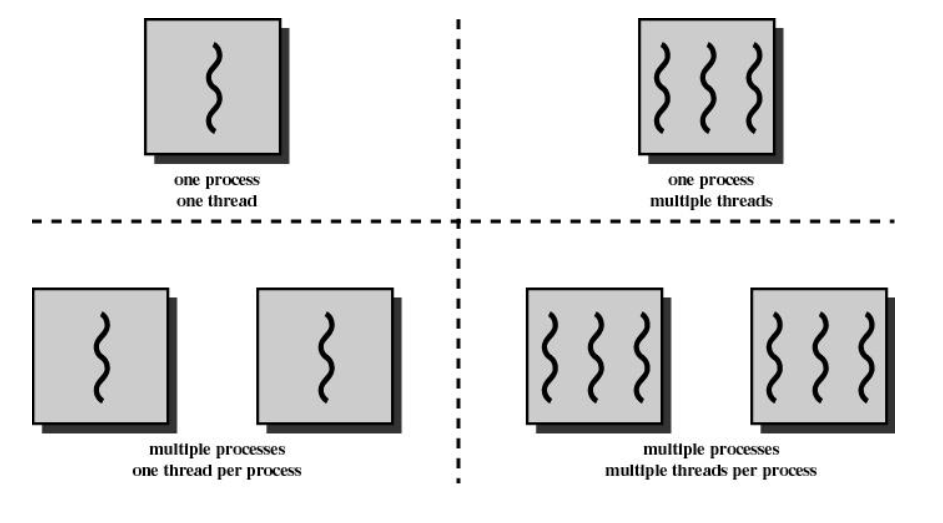
\includegraphics[scale=0.6]{img/C2/2-3/1.png}
	\caption{进程与线程的区别}
\end{figure}

由于线程比进程更小,基本上不拥有系统资源,故对它的调度所付出的开销就会小得多,能更高效的提高系统内多个程序间并发执行的程度,从而显著提高系统资源的利用率和吞吐量。因此使用线程可以带来很多好处:

\begin{itemize}
	\item 创建一个线程相比创建一个进程花费更少的时间。
	\item 结束一个线程相比结束一个进程花费更少的时间。
	\item 在同一个进程中切换不同线程花费更少的时间。
	\item 线程与资源分配无关,它属于某一个进程,与进程内其它线程一起共享进程资源。
\end{itemize}

\subsection{子进程(Child Process)}

\lstinline|fork()|函数是UNIX或类UNIX中的分叉函数,\lstinline|fork()|函数将运行着的程序分成两个几乎完全一样的进程,每个进程都启动一个从代码的同一位置开始执行的线程。这两个进程中的线程继续执行,就像是两个用户同时启动了该应用程序的两个副本。

\begin{lstlisting}[language=C, title=创建子进程]
#include <stdio.h>
#include <sys/types.h>
#include <wait.h>
#include <unistd.h>

int main() {
	pid_t pid;

	pid = getpid();
	printf("Before fork(): pid is %d\n", pid);

	// fork a child process
	pid = fork();

	if(pid < 0) {               // error
		fprintf(stderr, "Fork failed.\n");
		return 1;
	} else if(pid == 0) {       // child process
		printf("Child process: pid is %d\n", getpid());
		execlp("/bin/ls", "ls", NULL);
	} else {                    // parent process
		printf("Parent process: pid is %d\n", getpid());
		wait(NULL);
		printf("Child completed.");
	}
	
	return 0;
}
\end{lstlisting}

\begin{tcolorbox}
	\mybox{运行结果} \\
	Before fork(): my pid is 2250 \\
	Parent Process: my pid is 2250 \\
	Child Process: my pid is 2251 \\
	main main.c \\
	Child Complete
\end{tcolorbox}

\begin{figure}[H]
	\centering
	\begin{tikzpicture}[node distance=3cm,thick,auto]
		\node[state,initial] (fork) {fork};
		\node[state] (execvp)[below of=fork] {execvp};
		\node[state] (ls)[below of=execvp] {ls};
		\node[state] (wait)[right of=fork] {wait};
		\node[state,accepting below,accepting text = {end}] (end)[right of=ls] {end};

		\path[->] (fork) edge node[left] {child} (execvp);
		\path[->] (execvp) edge node {} (ls);
		\path[->] (ls) edge node {} (end);
		\path[->] (fork) edge node {parent} (wait);
		\path[->] (wait) edge node {} (end);
	\end{tikzpicture}
	\caption{子进程}
\end{figure}

正常情况下,子进程由父进程创建,子进程可以再创建新的进程。父子进程是一个异步过程,父进程永远无法预测子进程的结束,所以,当子进程结束后,它的父进程会调用\lstinline|wait()|或\lstinline|waitpid()|取得子进程的终止状态,回收掉子进程的资源。 \\

但是一些情况下会产生僵尸进程(zoobie process)和孤儿进程(orphan process)的情况:

\begin{itemize}
	\item 僵尸进程:子进程退出了,但是父进程没有用\lstinline|wait()|或\lstinline|waitpid()|去获取子进程的状态信息,那么子进程的进程描述符仍然保存在系统中,这种进程称为僵尸进程。
	
	\item 孤儿进程:父进程结束了,而它的一个或多个子进程还在运行,那么这些子进程就成为了孤儿进程。子进程的资源由init进程(pid=1)回收。
\end{itemize}

\newpage

\section{进程调度}

\subsection{进程调度(Scheduling)}

\begin{enumerate}
	\item 短程调度(STS, Short Term Scheduling):从准备队列中选择进程送到CPU执行。
	
	\item 中程调度(MTS, Medium Term Scheduling):从将外存中挂起的进程中选择进程送到内存。
	
	\item 长程调度(LTS, Long Term Scheduling):从外存中选择一个作业送到内存中,为其创建进程,并加入准备队列。
\end{enumerate}

\begin{figure}[H]
	\centering
	\begin{tikzpicture}[node distance=4.5cm,thick,auto]
		\node[state,initial] (s1) {New};
		\node[state] (s2)[below of=s1] {Ready};
		\node[state] (s3)[below of=s2] {Running};
		\node[state] (s4)[left of=s3] {Waiting};
		\node[state] (s4)[below of=s4] {Suspended};
		\node[state,accepting below,accepting text = {end}] (s4)[right of=s3] {Terminated};

		% \path[->] (s1) edge node[left] {admitted (LTS)} (s2);
		% \path[->] (s2) edge[bend left] node[above] {scheduler dispatch (STS)} (s3);
		% \path[->] (s3) edge[bend left] node[below] {interrupt} (s2);
		% \path[->] (s3) edge node[right] {I/O or event waiting} (s4);
		% \path[->] (s4) edge node[left] {swapping out (MTS)} (s5);
		% \path[->] (s3) edge node {终止} (s5);
	\end{tikzpicture}
	\caption{进程调度}
\end{figure}